\section{2DES auf gesättigten Heliumfilmen}
Wenn man in den Bereich des Phasendiagramms des 2DES vorstoßen will, in dem das 2DES als entartetes Elektronengas vorliegt, muss man Elektronendichten von $\gtrsim\unit[10^{15}]{\Em}$ erreichen. Derart hohe Elektronendichten sind, wie im vorigen Kapitel beschrieben auf Bulk"=Helium nicht stabil zu halten. Wenn man nun, wie schon in \cite{Ike81} vorgeschlagen, auf dünne Heliumfilme übergeht, kommt zusätzlich zur Stabilisierung durch die Gravitation die bei dünnen Filmen viel stärkere van"=der"=Waals"=Kraft zum tragen. In diesem Abschnitt sollen die Eigenschaften von Elektronen auf dünnen Heliumfilmen nun genauer untersucht werden.
 
\subsection{Allgemeine Eigenschaften}
\label{ssec:hefilm_allgemein}

\begin{figure}[h!tbp]
    \begin{center}
        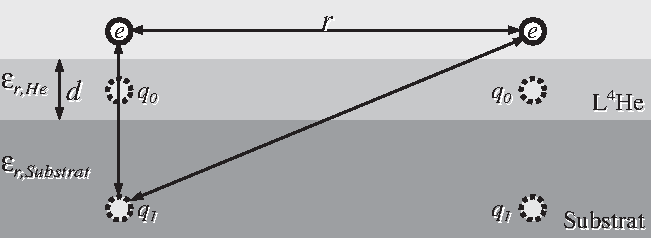
\includegraphics{theo_helium_filme/e_auf_filmen}
    \end{center}
    \caption[Wechselwirkungen auf dünnen Heliumfilmen]{Elektronen auf dünnen Heliumfilmen. Gezeigt ist schematisch wie die Wechselwirkung zwischen den Elektronen und den Bildladungen im Heliumfilm und Substrat zustande kommt. Der Charakter der $e$"=$e$"=Wechselwirkung wird durch die Abstände $d$ und $r$ bestimmt. Für $r\gg d$ ist die Wechselwirkung dipolartig, für $r\lesssim d$ Coulomb"=artig.}
    \label{eqn:film_schema}
\end{figure}

Der Übergang von 2DES auf Bulk"=Helium zu 2DES auf dünnen Heliumfilmen wird begleitet von der Änderung einiger Eigenschaften des Systems:

\begin{itemize}
    \item Der Heliumfilm ist aufgrund der starken van"=der"=Waals"=Wechselwirkung der Heliumatome mit dem Substrat stabil gegenüber der Aufweichung der Ripplonenmoden -- ganz im Gegensatz zur Oberfläche des Bulk"=Heliums. Die von dort bekannte elektrohydrodynamische Instabilität tritt hier nicht auf und als Folge davon kann der Heliumfilm weit höhere Elektronendichten tragen. Ob es hier eine obere Grenze für die Elektronendichte gibt, wurde in der Literatur \cite{Ike81,Etz84,Hu90} bereits diskutiert und wird in Abschnitt~\ref{ssec:film_stability} vorgestellt.
    \item Durch die im Vergleich zu Bulk"=Helium größere Dielektrizitätskonstante des Substrates folgt eine daraus resultierende stärkere Bildladung, so dass sich der coulombartige Charakter (hier $V\propto \frac1r$) der $e$-$e$"=Wechselwirkung für $r\gg d$ zunehmend in einen dipolartigen Charakter (mit $V\propto\frac1{r^3}$) wandelt. Dadurch wird die $e$-$e$-Wechselwirkung abgeschwächt, was zur Folge hat, dass das in Kapitel~\ref{sec:theo_phasendiagramm} vorgestellte Phasendiagramm eines 2DES modifiziert wird. Aufgrund der reduzierten $e$-$e$-Wechselwirkungsenergie verschiebt sich der Phasenübergang von der klassischen Elektronenflüssigkeit in den Wigner-Kristall zu höheren Elektronendichten hin. Der Quanten-Phasenübergang, der bei hohen Elektronendichten stattfindet, tritt bei kleineren Elektronendichten auf. Insgesamt schrumpft also der Bereich im Phasendiagramm, in dem ein Wigner-Kristall vorliegt. In Abbildung~\ref{fig:phase_diag_scheme} kann man das Phasendiagram von Bulk"=Helium mit dem von einem dünnen Heliumfilm auf Saphir und einem metallischen Substrat sehen. 
    \item Die Bindung der Elektronen an die Heliumoberfläche wird aufgrund der größeren Bildladung im dielektrischen Substrat stärker. Dies hat zur Folge, dass sich die Energieniveaus der Elektronen im 2DES zu tieferen Energien hin verschieben und sich der Abstand der Niveaus vergrößert.
    \item Bei dünnen Heliumfilmen muss zusätzlich auch der Einfluss der Oberflächenrauigkeit des Substrats berücksichtigt werden. Diese ist von Bedeutung, da alle im Experiment verwendeten Substrate eine Restrauigkeit besitzen. Man kann nicht mehr davon ausgehen, dass alle Elektronen frei sind, wie im sehr reinen System Elektronen auf Bulk"=Helium. Dies wird später noch bei der Behandlung des so genannten Zwei"=Komponenten"=Modells von Elektronen in Abschnitt~\ref{sec:theo_zweikomponenten} genauer diskutiert.
\end{itemize}

\subsection{Veränderung der Beweglichkeit auf dünnen He"=Filmen}

Im Vergleich zu den in Abbildung~\ref{fig:mobility} gezeigten Beweglichkeiten von Elektronen auf Bulk"=Helium von über $\unitfrac[10]{m^2}{V s}$ bei \unit[1.3]{K} bestimmten \name{Jiang} \ea \cite{Jia88} für Elektronen auf \unit[35]{nm} dicken Heliumfilmen bei \unit[1.3]{K} auf Glassubstrat eine Beweglichkeit von \unitfrac[2]{m$^2$}{V s} -- der theoretische Wert nach \name{Saitoh} \cite{Sai77} für freie Elektronen und ähnliche Bedingungen liegt bei \unitfrac[5]{m$^2$}{V s}.   
Auf dünnen Filmen bestimmten \name{Tress} \ea \cite{Tre96} die Beweglichkeit von Polaronen, also Elektronen, die sich mit einem Dimple fortbewegen, zu $<\unitfrac[1]{m^2}{V s}$.

Im Gegensatz zu Elektronen auf Bulk"=Helium hängt die Beweglichkeit von Elektronen auf dünnen Heliumfilmen sehr stark von der Qualität des verwendeten Substrates ab. Eine gute Vergleichbarkeit von Messungen an verschiedenen Substraten ist daher nur eingeschränkt gegeben.

\subsection{Verstärkung des von der Bildladung erzeugten Potentials}
Durch die Verwendung dielektrischer Substrate für die dünnen Heliumfilme erhält man eine durch die Spiegelladung im Substrat verursachte zusätzliche Komponente des Haltefeldes. 
Für die Parameter $n_s=\unit[10^{14}]{\Em}$, $d_\text{He-Gas}=\unit[5]{nm}$, $d_\text{He}=\unit[10]{nm}$ und $d_\text{Substrat}=\unit[200]{nm}$, die typisch für die durchgeführten Experimente sind, ergibt sich ein zusätzliches elektrisches Feld von ungefähr \unitfrac[500]{V}{mm}. Man kann sagen, dass das vom Substrat erzeugte Bildladungsfeld auf dünnen Heliumfilmen die Größenordnung des angelegten Haltefeldes erreicht. Dies ist der Grund für die in Abschnitt~\ref{ssec:saturation_film} gezeigte Hysterese der Beladekurve auf dünnen Heliumfilmen.
 
\subsection{Bestimmung der Elektronendichte auf dünnen Heliumfilmen}
\label{ssec:e_density}

Zur Berechnung der Abhängigkeit der Elektronendichte von dem bestimmenden Parameter -- der am Substrat angelegten Haltespannung -- wird eine Sammlung aus der Literatur bekannter Beziehungen benötigt, die hier kurz vorgestellt werden sollen:

\subsubsection{Abhängigkeit der Heliumfilmdicke vom Heliumstand}

Für die Dicke $d$ eines gesättigten Heliumfilms auf einem beliebigen Substrat gilt für den nicht retardierten Bereich für $d\lesssim\unit[100]{nm}$ folgende Gleichung:
    \begin{equation}
        \label{eqn:filmdicke}
        \frac{\DC k_\text{B}}{d_0^3}=\rho g h
            \qquad\Rightarrow\qquad
            d_0=\sqrt[3]{\frac{\DC\kB}{\rho g h}}\quad.
    \end{equation}

Der Parameter $\DC$, der die Stärke der van"=der"=Waals"=Wechselwirkung von Heliumatomen mit dem Substrat widerspiegelt, ist vom Substratmaterial abhängig.  
\begin{figure}[h!tbp]
    \begin{center}
        \raisebox{0.2cm}{%
        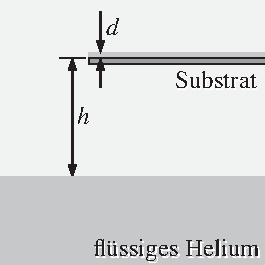
\includegraphics[width=3.5cm]{theo_helium_filme/saturated_films}} \quad
        \plotlink{filmdicke}{\includegraphics[width=\ssmallwidth]{theo_helium_filme/filmdicke}}
    \end{center}
    \caption[Filmdicke des Heliumfilms über der Bulk"=Flüssigkeit]{Abhängigkeit der Dicke des Heliumfilms von dem vertikalen Abstand zur Oberfläche des Bulk"=Heliums nach Gleichung~\eqref{eqn:filmdicke} für $\DC=\unit[26]{K}$. Nicht berücksichtigt ist hier die Retardierung des van"=der"=Waals"=Potentials für $d\gtrsim\unit[100]{nm}$.}
\end{figure}

Durch eine Variation der Filmdicke $d$, gesteuert durch den vertikalen Abstand $h$ der Bulk"=Helium"=Oberfläche vom Substrat, kann man somit die Dicke des Heliumfilms auf dem Substrat im experimentell zugänglichen Bereich von ca.\ \unit[25]{nm} bis zu mehr als \unit[90]{nm} variieren. Wie später noch gezeigt wird, verschwindet allerdings die Abhängigkeit der Filmdicke von der Höhe über der Oberfläche der Bulk-Flüssigkeit, wenn man zu größeren Elektronendichten übergeht. Dann üben die Elektronen einen so hohen Druck auf die Oberfläche des Heliumfilms aus, dass die Abhängigkeit vom vertikalen Abstand zum Bulk"=Helium keine Rolle mehr spielt.

\subsubsection{Änderung der Filmdicke bei Beladung mit Elektronen}

Der elektrostatische Druck, den die Elektronen auf die Oberfläche des Heliumfilms ausüben, wächst mit der Elektronendichte und der angelegten Haltespannung. Diese Kraft wird für Elektronendichten höher als \unit[10$^{13}$]{\Em} wichtig und führt dann zur Verringerung der Filmdicke des gesättigten Heliumfilms unter dem 2DES. Dieser Effekt wurde von \name{Etz} \ea~\cite{Etz84} mit Hilfe von Ellipsometrie an Heliumfilmen auf Substraten aus Glas und Silizium untersucht. Die Ergebnisse konnten mit folgender Abhängigkeit der Filmdicke von der gesättigten Elektronendichte $n_s$ und der Dicke des unbeladenen Heliumfilms $d_0$ gut beschrieben werden:
    \begin{equation}
        \label{eqn:beladene_filmdicke}
        d = d_0\left(1+\frac{n_s^2 e^2}{2\varepsilon_0\rho g h}\right)^{-\frac13}\quad.
    \end{equation}
%Siehe hierzu auch V. V. Tatarskii, N. I. Shikina and V. B. Shikin, Sov. Phys. JETP {\bfseries 55}, 444 (1982) und Sov. J Low Temp Phys. {\bfseries 10} No. 2 (1984). \TODO

\begin{figure}[h!tbp]
    \begin{center}
        \begin{minipage}[b]{\smallwidth}
        \plotlink{filmpressure}{\includegraphics[width=\smallwidth]{theo_helium_filme/filmpressure}}
        \end{minipage}
        \hfill
        \begin{minipage}[b]{\textwidth-\smallwidth-\tabcolsep}
            \caption[Beeinflussung der Filmdicke durch die Elektronendichte.]{Abhängigkeit der Dicke des Heliumfilms von der Elektronendichte in Sättigung nach Gleichung~\eqref{eqn:beladene_filmdicke} \cite{Etz84}. Die Anfangsfilmdicken $d_0$ sind $\unit[37]{nm}\;(h=\unit[5]{mm})$, $\unit[29.3]{nm}\;(h=\unit[10]{mm})$ und $\unit[23.3]{nm}\;(h=\unit[20]{mm})$.}\label{fig:filmdicke_elektronendichte}
        \end{minipage}
    \end{center}
\end{figure}

In Abbildung~\ref{fig:filmdicke_elektronendichte} ist gezeigt, wie sich die Dicke eines mit Elektronen beladenen Heliumfilms mit zunehmender Elektronendichte verringert. Hierbei wird deutlich, dass die Abhängigkeit der Filmdicke von ihrem Anfangswert ohne Elektronen bei hohen Elektronendichten immer geringer wird und bei Dichten größer als \unit[$4\times10^{14}$]{\Em} dann völlig verschwindet.
%TODO komischer Satz

\subsubsection{Abhängigkeit der Sättigungsdichte der Elektronen von der Filmdicke}
\label{sssec:theo_film_saettigung}

Nach den nun folgenden Überlegungen zur statischen Bestimmung der Elektronendichte folgt eine zur Bestimmung der wahren Elektronendichte wichtige selbstkonsistente Rechnung, die auch die Effekte der Reduzierung der Filmdicke durch den vorhandenen Elektronendruck berücksichtigt. Eine solche Methode wurde bereits in \cite{guenzler,Mis97} vorgeschlagen und verwendet, allerdings ohne dass die Vorgehensweise zur Berechnung der nach der Methode korrigierten Werte und auch die erhaltenen Ergebnisse diskutiert wurden.

In Analogie zum vorliegenden Experiment wird ein leitfähiges Substrat betrachtet, das mit einer isolierenden Deckschicht bedeckt ist. Ein schematischer Querschnitt durch die Substratoberfläche mit den in den Rechnungen verwendeten Bezeichnungen findet sich in Abbildung~\ref{fig:substrat_schema}. 
\begin{figure}[h!tbp]
	\begin{minipage}[b]{10cm}
		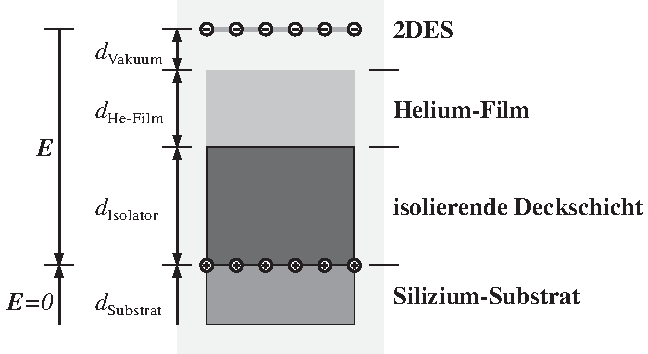
\includegraphics[width=10cm]{theo_helium_filme/electron_density}
	\end{minipage}\hfill
	\begin{minipage}[b]{\textwidth-10cm-\tabcolsep}
		\caption[Schema des Substrataufbaus zur Berechnung der Elektronendichte.]{Schematischer Schnitt durch die Substratoberfläche mit den in den Rechnungen verwendeten Größen. Gezeigt sind nur freie Ladungen und nicht die an den Grenzflächen der Dielektrika lokalisierten Verschiebungsladungen. $d_\text{Vakuum}$ ist der Gleichgewichtsabstand der Elektronen über der Heliumoberfläche von ca.\ \unit[100]{\AA}.}
	\label{fig:substrat_schema}
	\end{minipage}
\end{figure}

Die Elektronendichte in Sättigung wird definitionsgemäß erreicht, wenn der Raum oberhalb des 2DES feldfrei wird. Somit werden keine weiteren Elektronen durch das elektrische Feld angezogen und die Elektronendichte des 2DES bleibt konstant, obwohl das Filament weiter gepulst wird. Für diesen Fall kann man als Modell des Systems einen horizontal liegenden Plattenkondensator verwenden, dessen obere Platte das 2DES und die untere das leitfähige Silizium"=Substrat repräsentiert. Mit den folgenden bekannten Formeln für einen Plattenkondensator soll nun die Elektronendichte eines 2DES in Sättigung und in Abhängigkeit von der Haltespannung berechnet werden. Der Kondensator mit der Kapazität $C$ besitzt die Ladung $Q$ auf seinen Platten. Die Potentialdifferenz zwischen den Kondensatorplatten der Fläche $A$ ist $U$; $d$ ist der Abstand der Platten. Es gilt: 
\begin{equation}
    \label{eqn:plattenkondensator}
    Q=C\,U\textt{,}
    C=\varepsilon\frac{A}{d}\quad.
\end{equation}
Die Flächenladungsdichte $\nicefrac{Q}{A}$ des 2DES stimmt für den Fall der Beladung in Sättigung mit der Flächenladungsdichte der Elektronen am oberen Rand der leitfähigen Substratschicht überein. Da das 2DES aus dem Reservoir der angebotenen Elektronen schöpft, ohne dass ein zusätzliches Potential ein Rolle spielt, kann man annehmen, dass sich das 2DES wie eine mit der Masse verbundene Kondensatorplatte verhält und somit $U$ an der Kondensatorplatte der Haltespannung $U_\text{clamp}$ gleichsetzen. Die Elektronendichte in Sättigung des 2DES ergibt sich dann nach den Gleichungen~\eqref{eqn:plattenkondensator} zu
\begin{equation}
    \label{eqn:elektronendichte}
    n_s=\frac{Q}{e A}=
    \frac{U_\text{clamp}\varepsilon_0}{e}\frac1{
        \frac{d_\text{Vakuum}}{1}+
        \frac{d_\text{He-Film}}{\varepsilon_\text{r,He-Film}}+
        \frac{d_\text{Isolator}}{\varepsilon_\text{r, Isolator}}}\quad.
\end{equation}
Wie man sieht, ist in dieser einfachen Beziehung die Sättigungselektronendichte des 2DES $n_s$ proportional zur angelegten Haltespannung $U_\text{clamp}$. Aus der weiter unten folgenden selbstkonsistenten Korrektur für dünne Heliumfilme und hohe Elektronendichten ergeben sich dann Abweichungen von diesem linearen Verhalten.

Der mittlere Abstand der Elektronen zur Heliumoberfläche $d_\text{Vakuum}=\left<z\right>$ wird hier berücksichtigt, da sein Beitrag die Größe der Elektronendichte vor allem bei sehr dünnen Heliumfilmen beeinflusst. Die Abhängigkeit dieses Parameters von der Sättigungsfilmdicke wird hier nach der einfachen Näherung von \name{Hu} \ea\ \cite{Hu90} durch
\begin{equation}
	d_\text{Vakuum}\approx\left<z\right>\approx\unit[2]{nm} + 10^{-1}d
\end{equation}
bestimmt, die allerdings nur für Elektronen auf dünnen Heliumfilmen gültig ist.

\subsubsection{Selbstkonsistente Lösung zur Bestimmung der Elektronendichte}

Im Gegensatz zur Situation von sehr geringen Elektronendichten auf Bulk"=Helium ist die Bestimmung des Sättigungswertes der Elektronendichte auf dünnen Heliumfilmen durch die wechselseitige Abhängigkeit der Parameter Filmdicke $d$ und Elektronendichte $n_s$ erschwert. Gerade bei den hier auf Grund der van"=der"=Waals"=Stabilisierung des Heliumfilms erreichbaren höheren Elektronendichten werden die Abweichungen von einer einfachen Abschätzung nach Gleichung~\eqref{eqn:elektronendichte} ohne Berücksichtigung ihrer Filmdickenabhängigkeit signifikant.

Man kann nun versuchen, die reale Elektronendichte mit Hilfe einer selbstkonsistenten Rechnung aus den bereits bekannten Beziehungen~\eqref{eqn:elektronendichte} und \eqref{eqn:beladene_filmdicke} herzuleiten. Die Parameter, die die Elektronendichte und die Filmdicke dann bestimmen, sind
\begin{enumerate}
    \item die am Substrat angelegte Haltespannung $U_\text{clamp}$,
    \item der Höhenunterschied $h$ zwischen Substrat- und Bulk"=Helium"=Oberfläche und
    \item der Aufbau und die dielektrischen Eigenschaften der Substratoberfläche, $d_\text{Isolator},$ $\varepsilon_{r,\text{Isolator}}$, die dielektrischen Eigenschaften des Heliumfilms $\varepsilon_{r,\text{He-Film}}$ und die van-der-Waals Konstante von Helium auf dem Substrat $\DC$. 
\end{enumerate}

Als Startwert für die Filmdicke soll die Dicke des unbeladenen Heliumfilms dienen, wie sie sich aus Gleichung \eqref{eqn:filmdicke} ergibt. Für diese Filmdicke erhält man mit der gegebenen Haltespannung $U_\text{clamp}$ aus Gleichung~\eqref{eqn:elektronendichte} eine Elektronendichte $n_s(i=1)$ für die erste Iteration $(i=1)$. Wenn man nun nach Gleichung~\eqref{eqn:beladene_filmdicke} für die berechnete Anfangsfilmdicke und Elektronendichte $n_s(i=1)$ eine neue Filmdicke unter Elektronenbeladung $d(i=1)$ berechnet, kann man durch wiederholtes Einsetzen der erhaltenen Parameter in die Gleichungen~\eqref{eqn:elektronendichte} und \eqref{eqn:beladene_filmdicke} im Limes selbstkonsistente Werte für $d$ und $n_s$ erhalten:
\begin{equation}
    \begin{aligned}
        d(0) &= d_0\\[2ex]
        n_s(i+1) &= n_s\left(U,d(i), \ldots\right)\ttext{nach \eqref{eqn:elektronendichte}}\\
        d(i+1) &= d\left(d_0,n_s(i+1), \ldots\right)\ttext{nach \eqref{eqn:beladene_filmdicke}} \quad.
    \end{aligned}
\end{equation}
\begin{figure}[h!tbp]
    \centerline{\hfill%
        \subfigure[Konvergenz von $d$]{\plotlink{drec}{\includegraphics[width=\ssmallwidth]{theo_helium_filme/drec}}}\hfill%
        \subfigure[Konvergenz von $n_s$]{\plotlink{nrec}{\includegraphics[width=\ssmallwidth]{theo_helium_filme/nrec}}}\hfill%
    }
    \caption[Konvergenz der selbstkonsistenten Lösung]{Konvergenz der selbstkonsistenten Lösung der Sättigungsfilmdicke und der Sättigungselektronendichte für jeweils zwei Haltespannungen. Gezeigt ist die relative Änderung des berechneten Wertes für den jeweiligen Iterationsschritt.
(Parameter: $h=\unit[1]{cm}$, $d_\text{Substrat}=\unit[200]{nm}$, $d_\text{Vakuum}=\unit[10]{nm}$).}\label{fig:film_rekursion}
\end{figure}
Wie man in Abbildung~\ref{fig:film_rekursion} sehen kann, konvergieren die hierbei erhaltenen Parameter sehr schnell. Nach einigen Iterationen der hier vorgestellten Methode ändern sich die Werte von $d$ und $n_s$ nur noch geringfügig und man erhält eine gute Näherung für die wahre Filmdicke und Elektronendichte.

%TODO Rechtschreibung Weiteren groß/klein?
Im Weiteren wird immer eine zehnfache Iteration der hier vorgestellten Methode zur selbstkonsistenten Berechnung der Werte der Elektronendichte und Filmdicke Verwendung finden.

\subsubsection{Analyse der selbstkonsistenten Lösung}

\begin{figure}[h!tbp]
	\begin{center}
		\subfigure[Variation der Filmdicke]{\plotlink{uclamp_d_dep2}{\includegraphics[width=\smallwidth]{theo_helium_filme/uclamp_d_dep2}}}%
		\subfigure[Variation der Elektronendichte]{\plotlink{uclamp_n_dep2}{\includegraphics[width=\smallwidth]{theo_helium_filme/uclamp_n_dep2}}}
	\end{center}
	\caption[Elektronendichte auf PMMA, selbstkonsistente Rechnung]{Abhängigkeit {\bfseries (a)} der Elektronendichte $n_s$ und {\bfseries (b)} der Filmdicke $d$ von der angelegten Haltespannung $U_\text{clamp}$ nach selbstkonsistenter Rechnung. Parameter für PMMA: $h=$\unit[1]{cm}, $d_\text{Substrat}=$\unit[200]{nm}, $\varepsilon_\text{Substrat}=1.7$.}\label{fig:film_selbstkonsistent2}
\end{figure}

Der Verlauf von $d$ und $n_s$ in Abbildung~\ref{fig:film_selbstkonsistent2} für ein \unit[200]{nm} PMMA/Silizium"=Substrat zeigt den deutlichen Einfluss des Elektronendrucks auf die Filmdicke. Im Gegensatz dazu fällt die Korrektur zur Elektronendichte weitaus geringer aus und ist im Anbetracht der sonstigen Fehler bei der Bestimmung der Parameter, die der Elektronendichte zu Grunde liegen, zu vernachlässigen.

Der Einfluss auf die Elektronendichte wird für Elektronen auf einem \unit[200]{nm} \SiO/Silizium"=Substrat stärker, wie es in Abbildung~\ref{fig:film_selbstkonsistent} zu sehen ist. Der Einfluss der Änderung der Filmdicke durch den Elektronendruck auf \SiO"=Substrat wird schon bei sehr geringen Elektronendichten um $\unit[10^{14}]{\Em}$ merkbar und die Abweichung der Elektronendichte von der linearen Abhängigkeit von $U_\text{clamp}$ nach \eqref{eqn:elektronendichte} ist bei $U_\text{clamp}=\unit[2]{V}$ mehr als \unit[50]{\%}. Wie man sieht, geht die Dicke des Heliumfilms bei der maximalen Elektronendichte schon auf unter \unit[4]{nm}. Vor allem bei 2DES auf Substraten mit leitfähiger Oberfläche wird dieser Effekt der Filmdickenreduktion noch stärker sein. In diesem Bereich sind dann sehr glatte Substrate nötig, um das frühe Einsetzen des Tunnelns von Elektronen an Oberflächenrauigkeiten zu vermeiden. Dieser Effekt limitiert die maximal erreichbare Elektronendichte und soll später noch diskutiert werden. Aber auch bei Substraten, die eine isolierende Deckschicht besitzen, wird so der Einfluss der Oberflächenrauigkeit bei höheren Elektronendichten stärker. 
\begin{figure}[h!tbp]
	\begin{center}
		\subfigure[Variation der Filmdicke]{\plotlink{uclamp_d_dep}{\includegraphics[width=\smallwidth]{theo_helium_filme/uclamp_d_dep}}}%
		\subfigure[Variation der Elektronendichte]{\plotlink{uclamp_n_dep}{\includegraphics[width=\smallwidth]{theo_helium_filme/uclamp_n_dep}}}
	\end{center}
	\caption[Elektronendichte auf \SiO, selbstkonsistente Rechnung]{Abhängigkeit {\bfseries (a)} der Elektronendichte $n_s$ und {\bfseries (b)} der Filmdicke $d$ von der angelegten Haltespannung $U_\text{clamp}$ nach selbstkonsistenter Rechnung. Parameter für \SiO: $h=$\unit[1]{cm}, $d_\text{Substrat}=$\unit[200]{nm}, $\varepsilon_\text{Substrat}=4.5$.}\label{fig:film_selbstkonsistent}
\end{figure}

Unterschiedliche Substratmaterialien und die Art des Dielektrikums der Isolator"=Schicht haben, wenn man von der Güte der Substratoberfläche absieht, im Prinzip keinen Einfluss auf die erreichbaren Elektronendichten. Die Parameter der Isolierschicht $d_\text{Isolator}$ und $\varepsilon_{r,\text{Isolator}}$ ändern nur die lineare Skalierung der Abhängigkeit $n_s(U_\text{clamp})$; Kurvenscharen dieser Abhängigkeit liegen für verschiedene Sätze von Parametern der Isolierschicht übereinander. D.~h.\ der einzige Einfluss der Verwendung von Isolierschichten mit verschiedenem $\varepsilon_{r,\text{Isolator}}$ ist die im Abschnitt~\ref{ssec:phasediag_films} genauer beschriebene Modifikation des Phasendiagramms des 2DES.

\subsection{Stabilität des Heliumfilms bei hohen Elektronendichten}
\label{ssec:film_stability}

Verschiedene Autoren \cite{Ike81,Etz84,Hu90} kommen zu der Schlussfolgerung, dass dünne Heliumfilme auf dielektrischen Substraten bei sehr hohen Elektronendichten stabil bleiben. Nur die Wahrscheinlichkeit für das Tunneln von Elektronen durch die Barriere von \unit[1]{eV} nimmt mit dünner werdendem Film zu und muss vor allem bei Heliumfilmen auf leitfähigen Substraten beachtet werden.

Auf dünnen Heliumfilmen spielen zwei Effekte zur Stabilisierung/Destabilisierung der Filmoberfläche eine Rolle:
\begin{enumerate}
    \item der Deformationen der Oberfläche ausgleichende van"=der"=Waals"=Druck $\propto\frac1{d^4}$ und
    \item die Verstärkung der Bildladung bei zunehmender Dielektrizitätskonstante des Substrats.
\end{enumerate}
Ein Indikator für die Stabilität einer Heliumoberfläche gegenüber der Beladung mit Elektronen ist die Dispersionsrelation der Ripplonen.
Diese erhält, wie in \name{Ikezi} \ea{} \cite{Ike81} gezeigt, im Vergleich zur Situation auf Bulk"=Helium~\eqref{eqn:ripplon_dispersion_bulk} einen zusätzlich zur Erdbeschleunigung auftretenden, stabilisierenden van-der-Waals-Term $\frac{3\alpha}{\rho_\text{He} d^4}$. Für dünne Filme gilt:
    \begin{equation}
        \label{eqn:ripplon_dispersion:film}
        \omega^2_\text{ripplon}=\frac{\rho_s}{\rho_\text{He}}
			\left[\left(\frac{3\alpha}{\rho_\text{He} d^4}+g\right)k_\text{ripplon}+
            \frac{\sigma_\text{lv}}{\rho_He} k^3_\text{ripplon}-
			\frac{4\pi n^2e^2}{\rho_\text{He}} k^2_\text{ripplon}
				F(k_\text{ripplon},\varepsilon)\right]\tanh(k d)\quad.
    \end{equation}
Es wird angenommen, dass der Heliumfilm bis zur Sättigung mit Elektronen beladen ist und somit das elektrische Feld oberhalb der Elektronenschicht verschwindet. Die Funktion $F$ berücksichtigt die Auswirkung der Bildladung im Substrat. Für dielektrisches Material ist $F\approx\varepsilon$ und für Metalle gilt $F(d)=\coth(k_\text{ripplon}d)$.

Nach Analyse der Dispersionsrelation~\eqref{eqn:ripplon_dispersion:film} erhalten \name{Ikezi} \ea{} für \unit[10]{nm} Filmdicke eine untere Grenze  von \unit[$10^{15}$]{\Em} für die Instabilität. Des Weiteren weisen sie auf das Problem des Tunnelns von Elektronen bei diesen dünnen Filmen und hohen Haltefeldern hin.

Experimente zur Stabilität von Heliumfilmen auf verschiedenen Substraten wurden von \name{Etz} \ea{} \cite{Etz84} durchgeführt. Hierbei wurden Elektronendichten höher als \unit[$10^{15}$]{\Em} erfolgreich erzeugt. Allerdings zeigte sich bei den Messungen mit leitfähigem Silizium"=Substrat, dass die durch den Elektronendruck verursachte Reduzierung der Filmdicke nach Beenden der Beladung sofort wieder in Richtung des Startwertes relaxiert. Dies wird als Hinweis auf das Tunneln von Elektronen an Spitzen der Substratrauigkeit gesehen.

\subsubsection{Stabilitätskriterien}
Eine weitergehende Analyse der Stabilität von hohen Elektronendichten auf dünnen Heliumfilmen über verschiedenen Substraten wurde von \name{Hu} und \name{Dahm} durchgeführt (\cite{Hu90} und \cite{Dah91}).

Bei metallischen Substraten ist die gesättigte Elektronendichte immer nahe an der Stabilitätsgrenze. Das Bildladungspotential ist invers von der Filmdicke abhängig, aber die zusätzliche Entfernung des Elektrons vom Substrat aufgrund der Nullpunktsschwingung der Elektronen reduziert das effektive Haltefeld soweit, dass der Heliumfilm stabil bleibt.

Eine Schlussfolgerung von \cite{Hu90} ist, dass in Sättigung mit Elektronen beladene Heliumfilme für alle Elektronendichten gegenüber Oberflächenfluktuationen stabil sind. Für Substrate mit leitfähiger Oberfläche steigt allerdings mit abnehmender Filmdicke die Tunnelwahrscheinlichkeit und verhindert eine weitere Erhöhung der Elektronendichte ab Heliumfilmdicken unter \unit[3.5]{nm}. Für metallische Substrate geben \name{Hu} und \name{Dahm} deshalb eine maximal erreichbare Elektronendichte von ungefähr $\unit[1.5\times10^{15}]{\Em}$ an. Zusätzlich merken sie an, dass die Oberflächenrauigkeit auf realen Substraten schon bei weit geringeren Elektronendichten zum Einsetzen von Tunnelprozessen führen wird und dies das Erreichen von hohen Elektronendichten unmöglich macht. Sie schlagen auch vor, durch Aufbringen eines dünnen Films von festem Wasserstoff mit der Dicke von einigen Monolagen das Tunneln von Elektronen in das Substrat zu verringern. Dadurch könnte man die maximal erreichbare Elektronendichte um etwa eine Größenordnung erhöhen -- dann wird allerdings wieder das Tunneln von Elektronen direkt in das Substrat relevant.
